% =============================================================================
% FILE NAME : chapter1.tex
% DEPARTMENT: University of Tuebingen
% AUTOR     : Paul Palomero Bernardo
% =============================================================================
% CONTENT   : Include for chapter "Introduction"
% =============================================================================
\begin{table}[H]
Introduction\ldots

\section{Number of pages}
  \centering
  \begin{tabular}{|c|c|c|c|} \hline
    \textbf{Type} & \textbf{Lower bound} & \textbf{Upper bound} & \textbf{Remark} \\ \hline
		\hline
    Bachelor & 35 & 65 & ideal $\leq$ 50 \\ \hline
    Master & 50 & 85 & ideal $\leq$ 70 \\ \hline
  \end{tabular}
  \caption{\underline{Recommendation} on the number of pages for the thesis.}
  \label{tab:page_count}
\end{table}

\section{Latex examples}
\Gls{mlp} example\cite{goodfellow_deep_2016}.
\begin{figure}[H]
	\centering
	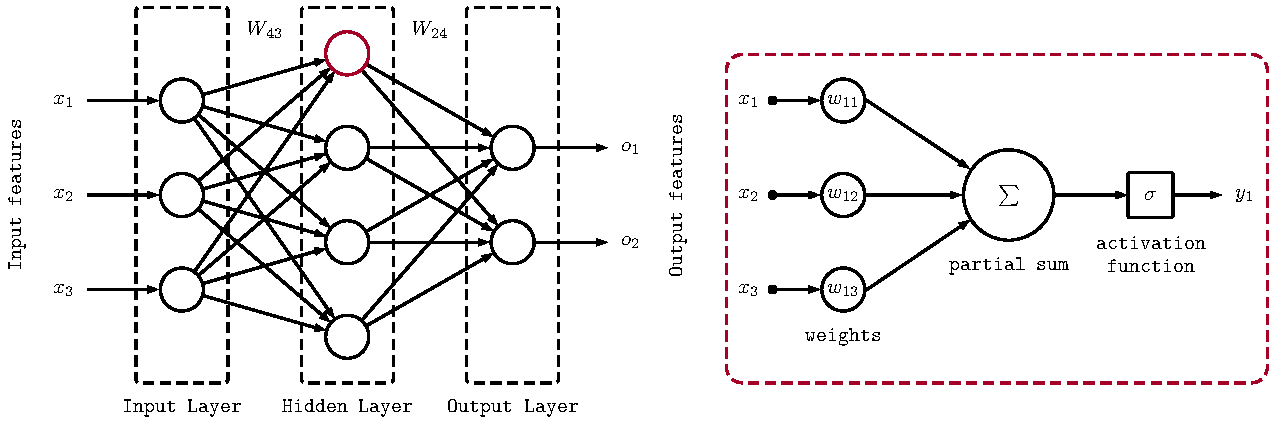
\includegraphics[width=\linewidth]{figures/example_fig.pdf}
	\caption[Schematic view of a simple MLP.]{Schematic view of a simple \gls{mlp}.}
  \label{fig:mlp}
\end{figure}

A website citation \cite{webpage}.

Using units \SI{32}{\bit}, \SI{64}{\kilo\byte}, \SI{3.14}{\milli\watt}.

\ifthenelse{\boolean{english}}{ENG}{GER}

\Blindtext